\section{Linguistic Linked Open Data} %: Building the Cloud}

Recent years have seen not only a number of approaches to provide linguistic data as Linked Data, but also the emergence of larger initiatives that aim at interconnecting these resources.
The \textbf{Open Linguistics Working Group (OWLG)}\footnote{\url{http://linguistics.okfn.org}} is an interdisciplinary network open to any individual interested in linguistic resources and/or the publication of these under an open license. The OWLG is a working group of the Open Knowledge Foundation (OKFN),\footnote{\url{http://okfn.org/}} a community-based non-profit organization promoting open knowledge (i.e., data and content that is free to use, re-use and to be distributed without restriction).
In this context, the Open Linguistics Working Group (OWLG) of the Open Knowledge Foundation (OKFN) has spearheaded the creation of 
new data and the republishing of existing linguistic resources as part of an emerging Linked Open Data (sub-) cloud of linguistic resources. 

This Linguistic Linked Open Data (LLOD) cloud is a result of a coordinated effort of the OWLG, its members and collaborating initiatives, most noteably the W3C Ontology-Lexica Community Group (OntoLex, see below) specializes in lexical-semantic resources.
As the OWLG organizes the LDL workshop series also as a vehicle to facilitate, to promote and to support this process, we would like to take the chance to unveil a revised cloud diagram on the occasion of LDL-2014.

\subsection{The LLOD Cloud}

In our current, informal understanding, \textbf{Linguistic Data} is pragmatically defined as any kind of resource considered relevant for linguistic research or Natural Language Processing tasks. 
Our assessment of relevance follows the classification of resources provided by data providers or the community, as reflected, for example, in tags assigned to resources at \url{datahub.io}, the meta data repository from which the LLOD cloud is currently being built. During diagram compilation, resources associated with the OWLG, or with tags like `LLOD', `linguistics', etc. are gathered, stored in a JSON document, categorized according to manually defined classification rules, and plotted and reformatted using a GraphML editor.\footnote{
	The extraction scripts can be found under \url{https://github.com/jmccrae/llod-cloud.py}.
}

Among these data sets, we encourage the use of \textbf{open} licenses and limit the diagram to such data sets. As defined by the Open Definition, ``openness'' refers to ``[any] piece of content or data [that] is open if anyone is free to use, reuse, and redistribute it -- subject only, at most, to the requirement to attribute and share-alike.''\footnote{\url{http://opendefinition.org}}

Linguistic \textbf{Linked} Open Data, then, comprises resources that are provided under an open license and published in conformance with the Linked Data principles as stated above.
Typically, these do not represent resources which are RDF-native, but resources that have been transformed into Linked Data. 

This also has an impact on the types of linguistic resources considered here, in particular the concept of \textbf{corpora}:
In empirical linguistics and NLP, \emph{collections of primary data} represent the elementary foundation of research and development. 
Yet, while it is possible to represent primary data such as plain text in RDF, this is not necessarily the most efficient way of doing so -- also given the fact that specialized XML-based standards such as the Text Encoding Iniative\footnote{
	\url{http://www.tei-c.org}
}
are well-established and widely used.
However, RDF provides highly flexible data structures that can be employed to represent linguistic annotations of arbitrary complexity. 
As understood \emph{here}, a `corpus' is thus always a linguistically analyzed resource:
Along with classical representations where both annotations \emph{and} primary data are modeled in RDF (e.g., in the seminal study of \citep{burchardt2008formalising}), 
but also hybrid data sets where only annotations are provided as Linked Data, but the primary data is stored in a conventional format (e.g., \citep{cassidy2010rdf}).
At the moment, corpora in the LLOD cloud seem to be relatively rare (see `\textsc{corpus}' resources in Fig.\ \ref{figI18nLOD}), 
but this only reflects the fact that several corpora had to be excluded from the diagram because they were not linked yet with other LLOD data sets such as lexical resources or repositories of annotation terminology.

Beyond representing linguistic analyses for collections of examples, text fragments, or entire discourses, 
the Linked Data paradigm particularly facilitates the management of \textbf{information about language and language resources} (`\textsc{metadata}' in Fig.\ \ref{figI18nLOD}).
These include linguistic databases (collections of features and inventories of individual languages, e.g., from linguistic typology), repositories of linguistic terminology (e.g., grammatical categories or language identifiers), and metadata about language resources (incl. bibliographical data).
While bibliographical data and terminology management represent classical Linked Data applications, our \emph{databases} are a specifically linguistic resource:
Databases of features of individual languages are a particularly heterogeneous group of linguistic resources; they contain complex and manifold types of information, e.g., feature structures that represent typologically relevant phenomena, along with examples for their illustration and annotations (glosses) and translations applied to these examples (structurally comparable to corpus data), or word lists (structurally comparable to lexical-semantic resources). RDF as a generic representation formalism is thus particularly appealing for this class of resources.

The third major group of resources in the diagram are \textbf{lexical-semantic resources} (`\textsc{lexicon}', \ref{figI18nLOD}), i.e., resources focusing on the general meaning of words and the structure of semantic concepts. 
These represent by far the most established type of linguistic resources in the LD context: They have been of inherent interest to the Semantic Web community, and hence a long tradition in this regard, going back to earliest attempts to integrate WordNet into the SW world \citep{gangemi2003ontowordnet}. 
In the diagram, we distinguish two types of lexical-semantic resources, i.e., \emph{lexical resources} in a strict sense (which provide specifically linguistic information, e.g., grammatical features, as found, e.g., in a dictionary, or in a WordNet), and and \emph{general knowledge bases} (such as classical thesauri or semantic repositories such as YAGO and DBpedia) 
whose origins lay outside of the stricter boundaries of linguistics or NLP. 
While the latter do not provide us with grammatical information, they formalize semantic knowledge, and in this respect, they are of immanent relevance for Natural Language Processing tasks such as Named Entity Recognition or Anaphora Resolution. 

\begin{figure*}[t]
 \begin{center}
% \includegraphics[width=0.97\textwidth]{images/LODLinguistics.jpg}
% \includegraphics[width=0.97\textwidth]{images/llod}
 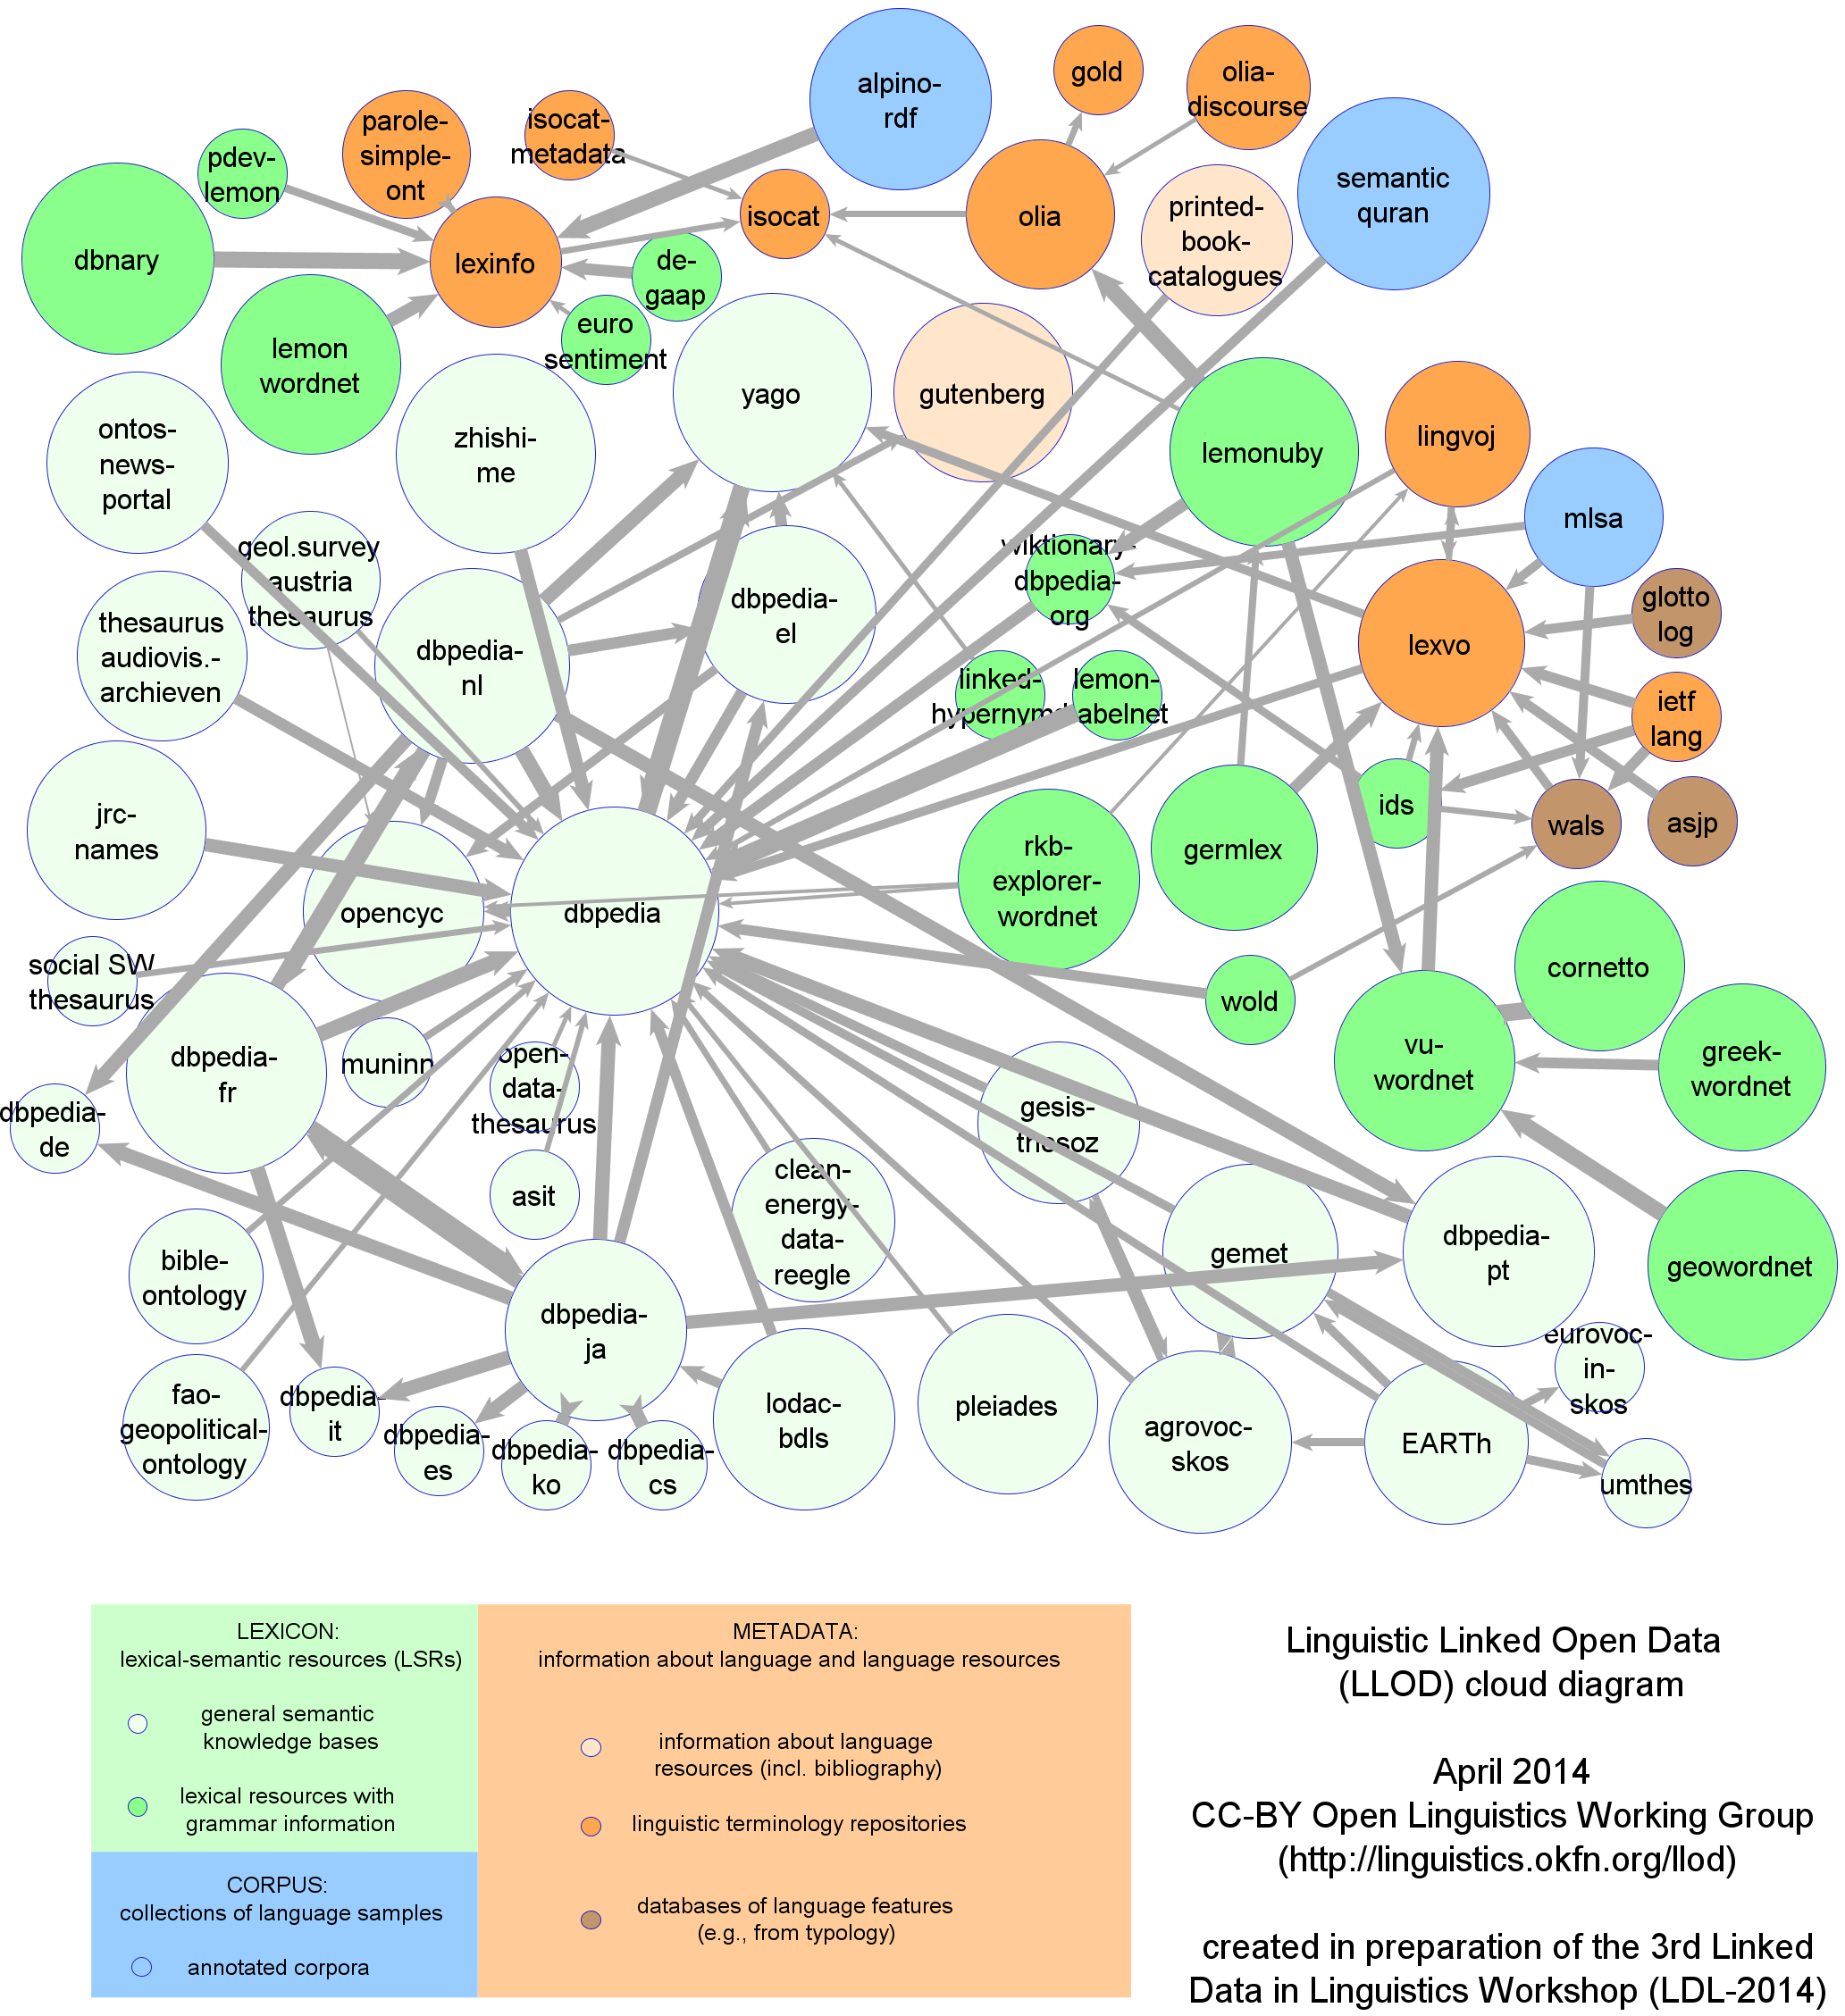
\includegraphics[width=1.0\textwidth]{llod-colored.png}
 \end{center}
\caption{Linguistic Linked Open Data cloud as of April 2014.}
\label{figI18nLOD}
\end{figure*}

\subsection{Recent Developments}

Since the publication of the last LLOD cloud diagram at LDL-2013, Sep 2013 in Italy, Pisa, we have continued to gather and to convert data sets, to refine our classification of language resources and encouraged others to contribute, e.g., by organizing LDL-2014 and the associated data challenge (see below).

These efforts have met with success such that the number of candidate resources for the cloud has increased substantially, from 65 resources in September 2013 to 107 in April 2014. 
We thus enforced the constraints imposed on resources in the cloud diagram. As of April 2014, we limit datasets in the cloud diagram to those with links to other LLOD data sets. 
Applying these stricter filters, we arrive at 68 resources in the new diagram.
For generating the diagram, we rely on the metadata as provided by Datahub.io, so only datasets are considered whose links with other LLOD data sets are explicitly documented there.
During diagram generation, we test whether the URLs given for the data are responding. At the moment, we do not, however, validate the information provided there, but a stricter validation routine is envisioned. 

Among others, novel data sets include resources prepared for LDL-2014 and the data challenge, but also resources that have not been covered by earlier diagram instantiations because they lacked the necessary tags to recognize them as being linguistically relevant. An example for the latter is the Greek WordNet (RDF edition released in early 2013),\footnote{
	\url{http://datahub.io/de/dataset/greek-wordnet}, cf. \url{http://okfn.gr/2013/01/983/}.
}
but also several thesauri and multilingual vocabularies.
This partially explains the growth of the cloud particular with respect to lexical resources. 

At the same time, the growing number of linked lexical resources also reflects the activities of the W3C Ontology-Lexica Community Group (OntoLex). The OntoLex group is not only closely collaborating with the OWLG, but both also have a considerable overlap in terms of their members, and as for LDL-2013, several LDL-2014 organizers are active in both groups.
While the OWLG is interested in open linguistic resources in general, the OntoLex group takes a specific focus on lexical resources, culminating in the proposal of a common model for machine-readable lexicons in RDF, the \emph{lemon} model \cite{mccrae2012integrating}. 
By now, already 41\% of lexical resources (7 out of 17) in the diagram (lemonWordNet, PDEVlemon, Parole/Simple, lemonUby, lemonBabelNet, germlex, DBnary) employ \emph{lemon} or \emph{lemon}-derived vocabularies, so that we see a considerable degree of convergence in this field. 
The resulting degree of interoperability and visibility arising from the use of shared vocabularies is certainly one of the most concrete achievements of the community activities we aimed to initiate with forming the OWLG, preparing the LLOD diagram and conducting workshops at linguistic, NLP and IT conferences.

\subsection{Organizing LDL-2014}

The LDL workshop series and LDL-2014 are organized by the Open Linguistics Working Group 
to bring together researchers from various fields of linguistics, NLP, and IT to present and discuss principles, case studies, and best practices for representing, publishing and linking linguistic data collections, and aims to facilitate the exchange of technologies, ideas and resources across discipline boundaries, that (to a certain extend) find a material manifestation in the emerging LLOD cloud.

LDL-2014, collocated with the 9th International Conference on Language Resources and Evaluation (LREC-2014), May 2014, Reykjavik, Iceland, is the third workshop on Linked Data in Linguistics following LDL-2012 (March 2012 in Frankfurt am Main, Germany), LDL-2013 (Sep 2013 in Pisa, Italy), as well as more specialized events such as the workshops on Multilingual Linked Open Data for Enterprises (MLODE-2012: Sep 2012 in Leipzig, Germany), and Natural Language Processing and Linked Open Data (NLP\&LOD-2013: Sep 2013 in Hissar, Bulgaria), and the theme session on Linked Data in Linguistic Typology (at the 10th Biennial Conference of the Association for Linguistic Typology, ALT-2013, Aug 2013 in Leipzig, Germany), as well as presentations, panels and informal meetings at various conferences.

LDL-2014 is organized in the context of two closely related community efforts, the \emph{Open Linguistics Working Group} (OWLG), and the \emph{W3C Ontology-Lexica Community Group} (OntoLex), and supported by two recently started EU projects, \emph{LIDER}, and \emph{QTLeap}.

The \textbf{Open Linguistics Working Group} was founded in October 2010, and since its formation, it has grown steadily. One of our primary goals is to attain openness in linguistics through:

\begin{enumerate}
\item Promoting the idea of open linguistic resources,
\item Developing the means for the representation of open data, and
\item Encouraging the exchange of ideas across different disciplines.
\end{enumerate}

The OWLG represents an open forum for interested individuals to address these and related issues.
At the time of writing, the group consists of about 130 	% that's a very conservative estimate, as of April 5, 2014, we have 185 subscribers 
															% (but there are a few duplicates, a few pseudo-addresses with purely technical 
															% function, and 2 unsubscriptions)
people from 20 												% that's an old estimate, not checked
different countries.
Our group is relatively small, but continuously growing and sufficiently heterogeneous. 
It includes
people from library science, typology, historical linguistics, cognitive science, computational linguistics, and information technology; the ground for fruitful interdisciplinary discussions has been laid out.
One concrete result emerging out of collaborations between a large number of OWLG members is the LLOD cloud as already sketched above.

The emergence of the LLOD cloud out of a set of isolated resources was accompanied and facilitated by a series of \textbf{workshops and publications} organized by the OWLG as sketched above. 
Plans to create a LLOD cloud were first publicly announced at LDL-2012, and subsequently, a first instance of the LLOD materialized as a result of the MLODE-2012 workshop, its accompanying hackathon and the data postproceedings that will appear as a special issue of the Semantic Web Journal (SWJ). 
The Second and Third Workshop on Linked Data in Linguistics continued this series of workshops.
In order to further contribute to the integration of the field, their organizers involved members of both the OWLG and the W3C Ontology-Lexica Community Group.

The \textbf{Ontology-Lexica Community (OntoLex) Group}\footnote{\url{http://www.w3.org/community/ontolex}} was founded  in September 2011 as a W3C Community and Business Group. It aims to produce specifications for a lexicon-ontology model that can be used to provide rich linguistic grounding for domain ontologies.
Rich linguistic grounding include the representation of morphological, syntactic properties of lexical entries as well as the syntax-semantics interface, i.e., the meaning of these lexical entries with respect to the ontology in question. An important issue herein will be to clarify how extant lexical and language resources can be leveraged and reused for this purpose. As a byproduct of this work on specifying a lexicon-ontology model, it is hoped that such a model can become the basis for a web of lexical linked data: a network of lexical and terminological resources that are linked according to the Linked Data Principles forming a large network of lexico-syntactic knowledge.

The OntoLex W3C Community Group has been working on realizing a proposal for a standard ontology lexicon model, currently discussed under the the designation \emph{lemon}. By now, the core specification of the model is almost complete, the group started to develop additional modules for specific tasks and use cases, and some of these are presented at LDL-2014.

As mentioned above, LDL-2014 is supported by two recently started EU Projects.
The project \textbf{Linked Data as an Enabler of Cross-Media and Multilingual Content Analytics for Enterprises Across Europe} (LIDER) aims to provide an 
ecosystem for the establishment of linguistic linked open data, as well as media resources metadata, for a free and open exploitation of such resources in 
multilingual, cross-media content analytics across Europe. 
The project \textbf{Quality Translation with Deep Language Engineering Approaches} (QTLeap) explores novel ways for attaining machine translation of higher quality that are opened by a new generation of increasingly sophisticated semantic datasets (including Linked Open Data) and by recent advances in deep language processing.

To accomodate the importance of multilinguality and semantically-oriented NLP that we encounter in the community as well as these initiatives, LDL-2014 takes a focus on Multilingual Knowledge Resources and Natural Language Processing, although contributions on Linked Data emphasising other aspects of linguistics or NLP were explicitly encouraged.